
\documentclass[9pt]{beamer}


%\usepackage[ngerman]{babel}
\usepackage{xspace}
\usepackage{pgf}
\usepackage{amssymb}
\usepackage{pifont}
\usepackage{color, colortbl}
\usepackage{subfigure}
\usepackage{tikz}
\usepackage[boxed, vlined, linesnumbered]{algorithm2e}

\usetheme{PaloAlto}

\usetikzlibrary{matrix,positioning,mindmap,automata,fit,backgrounds,
shapes, arrows,petri,calc, decorations.pathreplacing}

%

\newcommand{\FLTL}{\textrm{FLTL}\xspace}
\newcommand{\LTL}{\textrm{LTL}\xspace}

\newcommand{\AP}{\mathrm{AP}}  %
\newcommand{\cL}{\mathcal{L}}
\newcommand{\lattice}{\cL}

\newcommand{\logic}{\mathfrak{L}}
\newcommand{\SemL}[2]{{[#1 \models #2]_{\logic}}}
\newcommand{\Sem}[2]{{[#1 \models #2]}}
\newcommand{\SemF}[2]{{[#1 \models #2]_F}}
\newcommand{\SemFF}[2]{{[#1 \models #2]_4}}
\newcommand{\SemT}[2]{{[#1 \models #2]_3}}
\newcommand{\SemRV}[2]{{[#1 \models #2]_{RV}}}
\newcommand{\SemFf}[3]{{[#1,#2 \models #3]_{F}}}
\newcommand{\SemRVf}[3]{{[#1,#2 \models #3]_{RV}}}
\newcommand{\SemTf}[3]{{[#1,#2 \models #3]_3}}
\newcommand{\Semf}[3]{{[(#1,#2) \models #3]}}
%
\newcommand{\SemW}[2]{{[#1 \models #2]_{-}}}
\newcommand{\SemS}[2]{{[#1 \models #2]_{+}}}
\newcommand{\SemSW}[2]{{[#1 \models #2]_{\pm}}}
\newcommand{\SemWS}[2]{{[#1 \models #2]_{\mp}}}
\newcommand{\SemLTL}[2]{{[#1 \models #2]_{\omega}}}

\newcommand{\semExp}[2]{{\mathtt{ftl4}(#1,#2)}}
\newcommand{\fltlRew}[2]{{\mathtt{fltlRew}(#1,#2)}}


\newcommand{\Def}[1]{\alert{#1}}

\newcommand{\cA}{{\mathcal{A}}}
\newcommand{\cF}{{\mathcal{F}}}

\newcommand{\cM}{{\mathcal{M}}}
\newcommand{\BA}{\mathrm{BA}}
\newcommand{\NFA}{\mathrm{NFA}}
\newcommand{\DFA}{\mathrm{DFA}}
\renewcommand{\phi}{\varphi}

\newcommand{\true}{\ensuremath{\mathit{true}}\xspace} 
\newcommand{\false}{\ensuremath{\mathit{false}}\xspace}
\newcommand{\X}{\mathit{X}}
\newcommand{\nX}{\bar{\X}}    %
\newcommand{\U}{\mathrel{\mathit{U}}} %
\newcommand{\R}{\mathrel{\mathit{R}}} %

\newcommand{\sem}[1]{\ensuremath[\![#1]\!]}
\newcommand{\junit}{jUnit\xspace}
\newcommand{\junitrv}{jUnit$^{\mathrm{RV}}$\xspace}
\newcommand{\ltl}{\textrm{LTL}\xspace}

\newcommand{\WX}{\ensuremath{\operatorname{\overline{X}}}\xspace}
\newcommand{\G}{\ensuremath{\operatorname{G}}\xspace}
\newcommand{\F}{\ensuremath{\operatorname{F}}\xspace}
\renewcommand{\S}{\ensuremath{\operatorname{S}}\xspace}

\newcommand{\Until}{\mathit{U}}
\newcommand{\Release}{\mathit{R}}
\renewcommand{\complement}[1]{{\overline{#1}}}

\newcommand{\pbot}{{\bot^p}}
\newcommand{\ptop}{{\top^p}}
\newcommand{\meet}{\sqcap}
\newcommand{\join}{\sqcup}

\newcommand{\dual}[1]{\overline{#1}}


\renewcommand{\phi}{\varphi}
\newcommand{\nphi}{{\neg\phi}}

\newcommand{\monitor}{\ensuremath{{\sf monitor}}\xspace}
\newcommand{\step}{\ensuremath{{\sf step}}\xspace}
\newcommand{\decide}{\ensuremath{{\sf decide}}\xspace}

\newcommand{\emptiness}{\ensuremath{\text{\sf non-empty}}\xspace}

\newcommand{\extrapolate}{\ensuremath{{\sf extrapolate}}\xspace}
\newcommand{\abstractfct}{\ensuremath{\alpha}}

\lstdefinelanguage{forLTL}
{morekeywords={
  let, in, true, false,
  always, historically, alwaysinpast,
  between, betweeninpast,
  eventually, once, eventuallyinpast,
  from, after, frominpast,
  holding, holdinginpast,
  never, neverinpast,
  next, previous, nextinpast,
  nextn, previousn, nextninpast,
  occurring, occurringinpast,
  releases, triggered, releasesinpast,
  until, since, untilinpast,
  upto, before, uptoinpast,
  required, req, optional, opt, weak,
  inclusive, incl, exclusive, excl,
  and, or, implies, equals, not,
  if, then, else,
  rejecton, accepton,
  assert, declare, define,
  allof, someof, noneof, exactlyoneof,
  enumerate, list, as, in,
  with, without,
  timed,
  alw, even  %
},
sensitive=true,
morecomment=[l]{--},
morestring=[b]"
}

\lstset{frame=none, 
        basicstyle=\ttfamily, 
        keywordstyle=\bfseries, 
        mathescape=true,
        commentstyle=\color[gray]{0.5}, 
        breaklines=true, 
        breakatwhitespace=true,
        showstringspaces=false,
        xleftmargin=3ex
}

\newcommand{\Def}[1]{\alert{#1}}

\mode<presentation>{
\usetheme{McMaster}
\title{ Decentralized Crash-Resilient Runtime Verification}
\subtitle{}
\author[Shokoufeh Kazemlou]{\textcolor{blue}{\Large Shokoufeh Kazemlou}}
\institute{\large Department of Computing and Software \\ McMaster University}
\subject{Fault-tolerant Monitoring}
\keywords{}
\date{\today}
}

\mode<article>{
\usepackage{document}
\documentCourse{}
\documentAuthors{Shokoufeh Kazemlou}
\documentTerm{}
\documentDate{}
\documentTitle{Presentation at McMaster University}
\documentSubtitle{}
}

\iffalse
\AtBeginSubsection[]
{
  \begin{frame}<beamer>
    \frametitle{Outline}
    \tableofcontents[currentsection,currentsubsection]
  \end{frame}
}
\fi

\AtBeginSection[]{\frame{\frametitle{Presentation outline}\tableofcontents[current]}}

%\renewcommand{\cite}[1]{\textcolor{lightBlue}{[#1]}}

\newcommand{\I}[1]{\mathit{#1}}
\newcommand{\syntru}{\I{true}} %syntactical true
\newcommand{\synfals}{\I{false}} %syntactical false
\newcommand{\inftrace}{w}
\newcommand{\fintrace}{u}
\newcommand{\tru}{\mathit{true}}
\newcommand{\fals}{\mathit{false}}
\newcommand{\word}{w}
\newcommand{\emptyword}{\epsilon}
\newcommand{\alphabet}{\Sigma}
\newcommand{\LS}{\mathit{LS}}
\newcommand{\SM}{\mathit{SM}}
\newcommand{\TT}{{\top_p}}
\newcommand{\FT}{{\bot_p}}
\newcommand{\LTL}{{\sc Ltl}\xspace}
\newcommand{\LTLtri}{{\sc Ltl}$_3$\xspace}
\newcommand{\LTLk}{{\sc Ltl}$_K$\xspace}
\newcommand{\RVLTL}{{\sc Rv-Ltl}\xspace}
\newcommand{\FLTL}{{\sc Fltl}\xspace}
\newcommand{\LTLfour}{\RVLTL}%{{\sc Ltl}$_4$\xspace}
\newcommand{\zplus}{\mathbb{Z}_{\geq 0}}
\newcommand{\prog}{\mathcal{D}}
\newcommand{\AP}{\mathit{AP}}
\newcommand{\ap}{\mathit{ap}}
\newcommand{\F}{\mathbf{F}}
\newcommand{\G}{\mathbf{G}}
\newcommand{\X}{\mathbf{X}}
\newcommand{\U}{\mathbf{U}}
\newcommand{\udef}{\natural}
\newcommand{\monitor}{\mathcal{M}}
\newcommand{\trace}{\sigma}
\newcommand{\alltrace}{\mathrm{\Xi}}
\newcommand{\pred}{\mathcal{F}}
\newcommand{\AN}{\mathit{AN}}


\newcommand{\state}{s}





\newcommand{\Exltl}{Extended \LTLtri monitor}
\newcommand{\DSM}{decentralized synchronous monitoring}
\newcommand{\intersection}{\mathcal{I}^\monstate}
\newcommand{\verdict}{V}
\newcommand{\valuation}{\nu}
\newcommand{\pevent}{E}
\newcommand{\events}{states}
\newcommand{\event}{state}
\newcommand{\monstate}{q}
\newcommand{\correctverd}{\monstate_c}
\newcommand{\correctverdict}{correct verdict}
\newcommand{\truthvalue}{truth value}
\newcommand{\abstate}{LS}
\newcommand{\absfunc}{\mu}
\newcommand{\indisting}{indisting?}
\newcommand{\disting}{disting?}
\newcommand{\dep}{covered?}
\newcommand{\partition}{PARTITION}
\newcommand{\partitionn}{partition}
\newcommand{\splitt}{SPLIT}
\newcommand{\splt}{split}
%\newcommand{\snap}{Snap}
\newcommand{\snap}{\mathit{Snap}}
\newcommand{\indist}{indistinguishable}
\newcommand{\dist}{distinguishable}
\newcommand{\covered}{covered}
\newcommand{\localreg}{local snapshot}

\newcommand{\sample}{\mathcal{S}}
\newcommand{\ps}{\sample}



\tikzset{
  invisible/.style={opacity=0},
  visible on/.style={alt={#1{}{invisible}}},
  alt/.code args={<#1>#2#3}{%
    \alt<#1>{\pgfkeysalso{#2}}{\pgfkeysalso{#3}} % \pgfkeysalso doesn't change the path
  },
}


\iffalse
\usepackage{pgfpages}
\setbeamertemplate{note page}[plain]
\setbeameroption{show notes on second screen=right}
\fi

\setbeamertemplate{footline}[frame number]


\graphicspath{{figures/}}

\pgfdeclarelayer{background}
\pgfdeclarelayer{foreground}
\pgfsetlayers{background,main,foreground}

\tikzset{
  invisible/.style={opacity=0, text opacity=0},
  visible on/.style={alt={#1{}{invisible}}},
  alt/.code args={<#1>#2#3}{%
    \alt<#1>{\pgfkeysalso{#2}}{\pgfkeysalso{#3}} % \pgfkeysalso doesn't change 
the path
  },
}


\tikzstyle{place}=[circle,thick,draw=blue!75,fill=blue!20,minimum size=6mm]
\tikzstyle{red place}=[place,draw=red!75,fill=red!20]
\tikzstyle{transition}=[rectangle,thick,draw=black, fill=black, 
minimum size=1mm]


\setbeamercolor{block body}{bg=cyan!5,fg=black}


\begin{document}

%\tikzset{%
  every state/.style={
    draw=maincolor,
    thick,
    fill=maincolor!18,
    inner sep=.8ex,
    minimum size=0pt
  },
  active/.style={
    draw=alertedcolor,
    fill=alertedcolor!18
  },
  bool/.style={
    state,
    shape aspect=2,
    shape=diamond
  },
  shorten >=1pt,
  initial text={},
  every initial by arrow/.style={thick},
  frame/.style={
    line width=.5ex,
    rounded corners=1ex,
    inner sep=1ex
  }
}

\xdefinecolor{maincolor}{RGB}{0, 120, 140}
\colorlet{alertedcolor}{purple}
\colorlet{examplecolor}{green!50!black}

\colorlet{Blue}{maincolor}
\colorlet{Red}{alertedcolor}
\colorlet{Green}{examplecolor}

%\lstdefinestyle{long}{basicstyle=\scriptsize\ttfamily}

\frame{\titlepage}
\mode<article>{\printDocumentHeader}

\iffalse
  \begin{frame}
  \frametitle<presentation>{Outline}
  \tableofcontents
  \end{frame}
\fi


\begin{frame}{Overview}
\tableofcontents
\end{frame}



\section{Motivation}

%-------------------------------------------------------------------------
\begin{frame}{Motivation}

\begin{block}{Traditional Verification}
 
\Def{Exhaustive verification} methods are extremely valuable to ensure 
system-wide correctness.


\note{RV complements exhaustive verification methods such as model checking and theorem proving, as well as incomplete solutions such as testing and debugging. Exhaustive verification often requires developing a rigorous abstract model of the system and suffers from the infamous state-explosion problem. Testing and debugging, on the other hand, provide us with under-approximated confidence about the correctness of a system as these methods only check for the presence of defects for a limited set of scenarios\\
\Def{Traditionally}, one considers three main verification techniques: theorem proving [12], model checking [20], and testing [49,16]. Theorem proving, which is mostly applied manually, allows to show correctness of programs similarly as a proof in mathematics shows correctness of a theorem. Model checking, which is an automatic verification technique, is mainly applicable to finite-state systems. Testing covers a wide field of diverse, often ad hoc, and incomplete methods for showing correctness, or, more precisely, for finding bugs..}

\ \\

They often require developing an abstract model of the system and may suffer 
from the 
infamous \Def{state-explosion} problem.


\end{block}

\pause

\begin{block}{Runtime Verification}
 
\Def{Runtime verification} (RV) refers to a technique, where a monitor checks 
at 
run time whether or not the execution of a system under inspection satisfies a 
given correctness property. 

\ \\

RV \Def{complements} exhaustive verification techniques as well as 
underapproximated methods such as testing and tracing.

\end{block}

\end{frame}

% ----------------------------------------------------------------------------
\begin{frame}{Motivation}

\begin{block}{RV in Distributed Systems}
 
Designing a \Def{decentralized runtime monitor} for a \Def{distributed
system} is an especially difficult task since it deals with

\begin{itemize}
 \item computing \Def{global snapshots} at run time, and 
 \item estimating the \Def{total order} of events
\end{itemize}

in order for the monitor to reason about the temporal behavior of the system.

\end{block}



\note{Abstraction Function in Automata-Based Algorithm. Here we define the abstract local state LSi of a monitor Mi to be the verdict set Vi emitted by the monitor. Given the concrete local state Sis of a monitor Mi and the Ltl3 monitor Mφ of an Ltl formula φ, the abstraction function first computes the set of possible global states E(Sis) from viewpoint of monitor Mi, and then calculates the verdict set based on E(Sis). More formally
}



\end{frame}

% ----------------------------------------------------------------------------



\section{\LTLtri Monitor}
\begin{frame}{3-Valued \LTL (\LTLtri) [Bauer, Leucker, Schallhart 11] }

3-valued \LTL evaluates \LTL formulas for finite words with an 
eye on \Def{possible future extensions}.

\ \\

%\pause

\begin{block}{Three Truth Values}
 
The set of truth values is \Def{$\mathbb{B}_3=\{\top,\bot, ?\}$}, where

\begin{itemize}

%\pause

 \item \Def{$\top$:} the formula is \Def{permanently satisfied} no matter 
how the current execution extends,

%\pause

\item \Def{$\bot$:} the formula is \Def{permanently violated} no matter 
how the current execution extends

%\pause

\item \Def{?:} denotes an unknown verdict; i.e., there exist extensions that can 
falsify or make true the formula.
\end{itemize}

\end{block}

\end{frame}

% ----------------------------------------------------------------------------



\begin{frame}{3-Valued \LTL}

\ \\

\begin{block}{\LTLtri Semantics}
Let $u \in \alphabet^{*}$ be a finite word. The truth value of an \LTLtri 
formula $\varphi$ with respect to $u$, denoted by $[u \models_3 \varphi]$, is 
defined as follows:

 \begin{equation*}
 	\left[ u \models_3 \varphi \right] = 
 		\begin{cases} \top & \text{if }~~~~~\forall w \in 
\alphabet^\omega : 
uw \models \varphi\\
 		\bot & \text{if }~~~~~\forall w \in \alphabet^\omega : uw \not 
\models \varphi\\
 		? & \text{otherwise}.
 	\end{cases}
 \end{equation*}
 
\end{block}

\end{frame}

% ----------------------------------------------------------------------------





\begin{frame}{3-Valued \LTL}

\begin{block}{\LTLtri Monitor}
 
Let $\varphi$ be an \LTL formula. The \Def{\LTLtri monitor} of $\varphi$ 
is the unique deterministic finite state machine $\monitor^{\varphi}_3 = 
(\alphabet, Q, q_0, \delta, \lambda)$, where $Q$ is a set of states, $q_0$ is 
the initial state, $\delta \subseteq Q \times \alphabet \times Q$ is the 
transition relation, and $\lambda: Q \rightarrow \mathbb{B}_3$, is a function 
such that:
\begin{equation*}
\lambda(\delta(q_0, u)) = \left[u \models_3 \varphi\right]
 \end{equation*} 
for every finite word $u \in \alphabet^*$. \qed

\end{block}

%\pause

\begin{example}{\LTLtri monitor for $a \, \U \, b$}

\vspace{-7mm}
 \begin{figure}
 \centering
 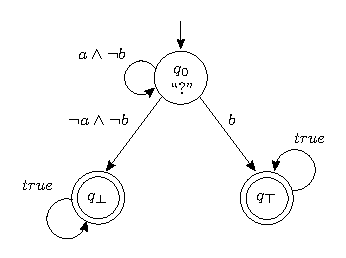
\includegraphics[scale=.85]{figures/exprop}
 \end{figure}

\end{example}

\end{frame}









\iffalse

\begin{frame}{\LTLtri}

\begin{example}

%\pause

\begin{tikzpicture}[->,>=stealth',shorten >=1pt,auto,node distance=2cm,
                    semithick]
 \tikzstyle{every state}=[draw=blue!75,fill=blue!10,minimum size=7mm]

\hspace{-1cm} $[u \models_3 \X p] = \top$ \hspace{1.5cm}
  \node[initial,initial text={}, state] (A) {};
  \node[state]         (B) [right of=A] {$p$};
  \node[state]         (C) [right of=B] {};
  \node[state]         (D) [right of=C] {};

  \path (A) edge node {} (B)
        (B) edge node {} (C)
        (C) edge node {} (D);
        
\end{tikzpicture}

%\pause

\vspace{.5cm}
\begin{tikzpicture}[->,>=stealth',shorten >=1pt,auto,node distance=2cm,
                    semithick]
 \tikzstyle{every state}=[draw=blue!75,fill=blue!10,minimum size=7mm]

\hspace{-1cm}  $[u \models_3 p \, \U \, q] = ?$ \hspace{1.2cm}

  \node[initial,initial text={}, state] (A) {$p$};
  \node[state]         (B) [right of=A] {$p$};
  \node[state]         (C) [right of=B] {$p$};
  \node[state]         (D) [right of=C] {$p$};

  \path (A) edge node {} (B)
        (B) edge node {} (C)
        (C) edge node {} (D);
        
\end{tikzpicture}

%\pause

\vspace{.5cm}

 \begin{tikzpicture}[->,>=stealth',shorten >=1pt,auto,node distance=2cm,
                    semithick]
 \tikzstyle{every state}=[draw=blue!75,fill=blue!10,minimum size=7mm]

\hspace{-1cm} $[u \models_F \F p] = \top$ \hspace{1.5cm}

  \node[initial,initial text={}, state] (A) {};
  \node[state]         (B) [right of=A] {};
  \node[state]         (C) [right of=B] {$p$};
  \node[state]         (D) [right of=C] {};

  \path (A) edge node {} (B)
        (B) edge node {} (C)
        (C) edge node {} (D);
        
\end{tikzpicture}

%\pause

\vspace{.5cm}

\begin{tikzpicture}[->,>=stealth',shorten >=1pt,auto,node distance=2cm,
                    semithick]
 \tikzstyle{every state}=[draw=blue!75,fill=blue!10,minimum size=7mm]

 \hspace{-1cm} $[u \models_F \G p] = \bot $ \hspace{1.5cm}

  \node[initial,initial text={}, state] (A) {$p$};
  \node[state]         (B) [right of=A] {$p$};
  \node[state]         (C) [right of=B] {$\neg p$};
  \node[state]         (D) [right of=C] {};

  \path (A) edge node {} (B)
        (B) edge node {} (C)
        (C) edge node {} (D);
        
\end{tikzpicture}
\end{example}
\end{frame}
\fi
% ----------------------------------------------------------------------------




% ----------------------------------------------------------------------------


\iffalse

\section{\LTLtri Monitor}
\begin{frame}{\LTLtri Monitor}

\begin{block}{3-Valued \LTL}

\begin{itemize}

\item The 3-valued semantics of \LTL (denoted \LTLtri) evaluates \LTL 
formulas for finite traces with an eye on possible future extensions. 
\item In \LTLtri, the set of truth values is $\mathbb{B}_3=\{\top,\bot, ?\}$
\end{itemize}

\end{block}

 \begin{block}{Example ($\varphi = a \, \U \, b$)}
  \begin{figure}
\centering
\begin{tikzpicture}[->,>=stealth',shorten >=1pt,auto,node distance=2.8cm, 
semithick, scale=.6, initial text={}, font=\small]
\node[state, accepting] (A)                    {$q_\bot$};
  \node[initial,state]         (B) [above right of=A] {$q_0$};
  \node[state, accepting]         (C) [below right of=B] {$q_\top$};
   
 \path  (B) edge [loop above] node  {$a \wedge \neg b$} (B)
        (B) edge node [left, yshift=2mm] {$\neg a \wedge \neg b$} (A)
        (B) edge node [right, yshift=2mm] {$b$} (C)
        (A) edge [loop below] node  {$\mathit{true}$} (A)
        (C) edge [loop below] node  {$\mathit{true}$} (C);
\end{tikzpicture}

\end{figure}
 \end{block}


\end{frame}
\fi


\section{Problem Statement}



\begin{frame}{Problem Statement}
 
\begin{block}{Distributed Monitors}
 
Let $\monitor = \{M_1, M_2, \ldots, M_n\}$ be a set of \Def{distributed 
monitors} monitoring an underlying system. 

\iffalse
Suppose $\alpha = s_0 s_1\cdots s_k$ is a finite trace 
generated by the system under inspection, and $\varphi$ is an \LTL formula.

\ \\

%\pause

Each monitor $M_i \in \monitor$ takes a sample \Def{only once} from the 
underlying system to obtain the values of propositions in $\AP$ as input.
\fi
\end{block}

\vspace{-10mm}
\begin{figure}
 \centering
 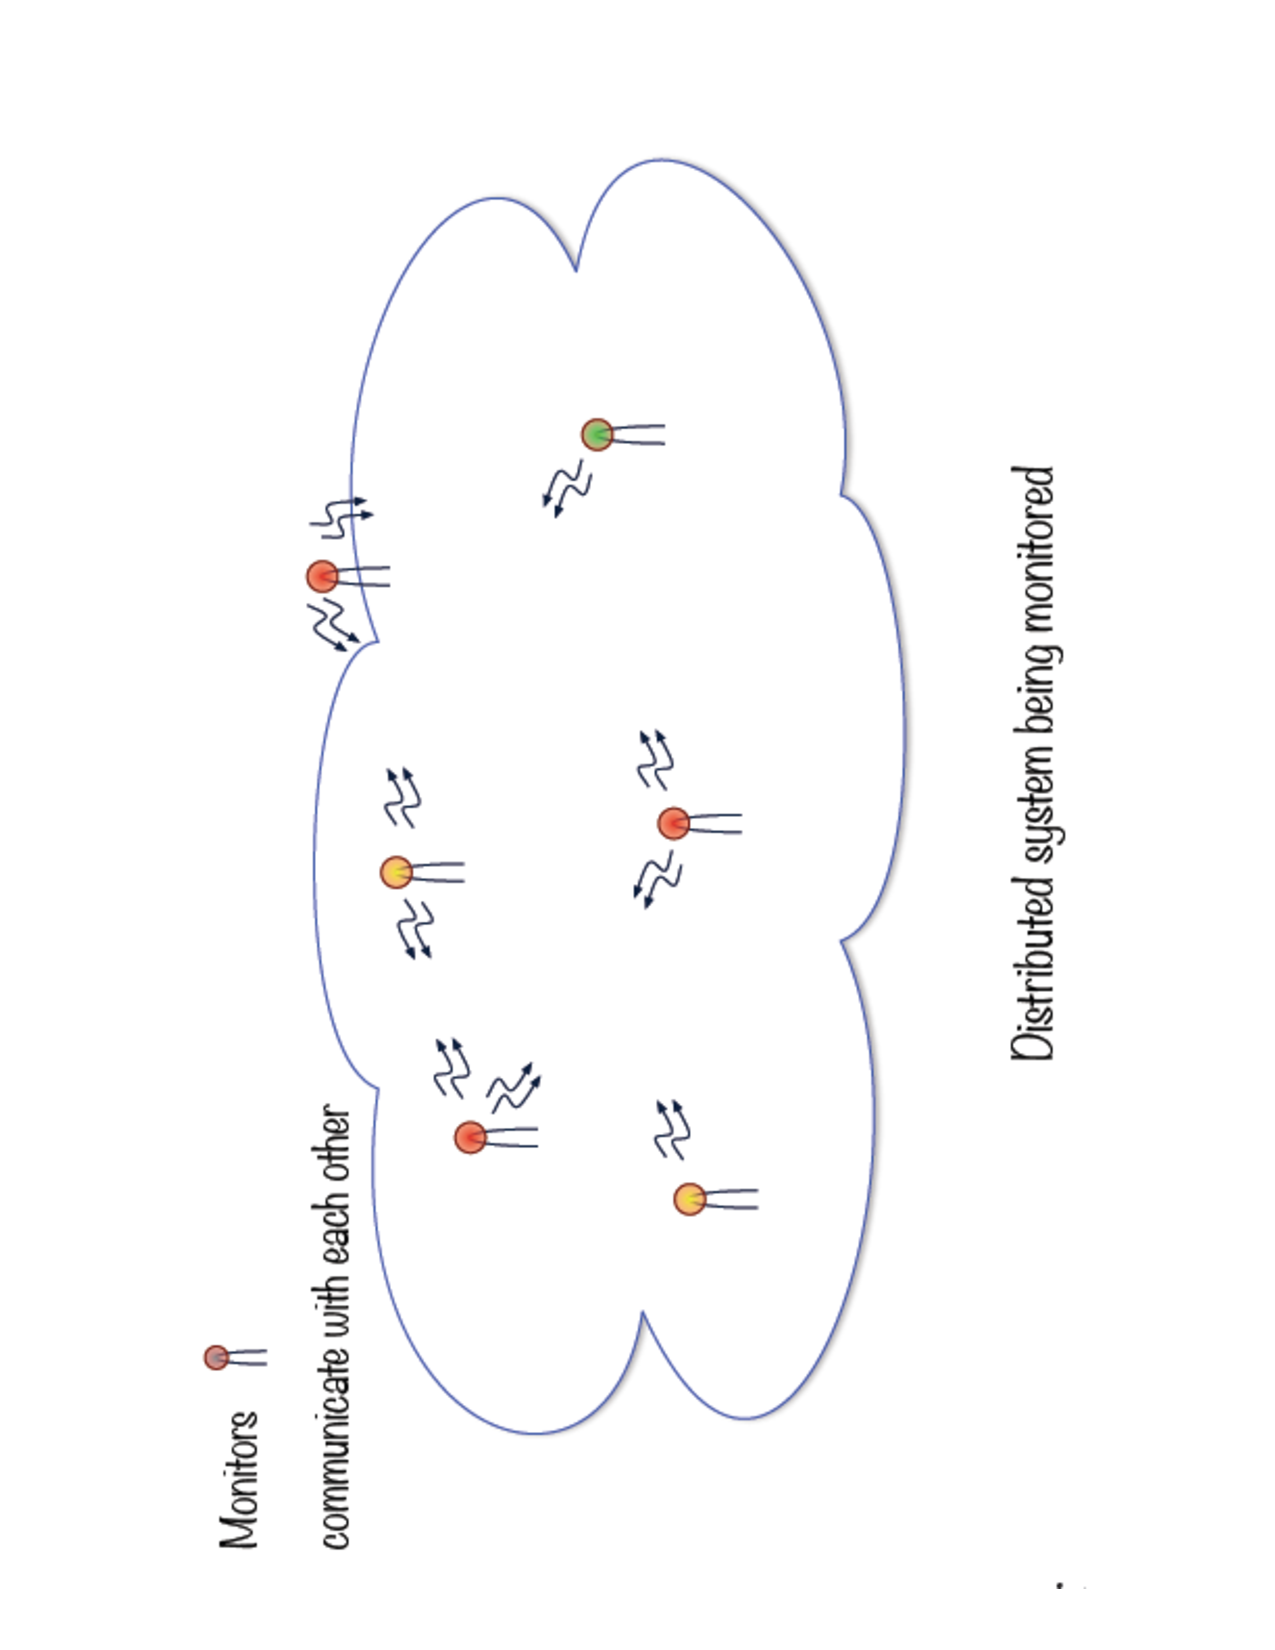
\includegraphics[scale=.29, angle=-90]{figures/wfdm}
 \end{figure}

\end{frame}
 
 % ----------------------------------------------------------------------------



\iffalse
\begin{frame}{Problem Statement}


\begin{block}{Synchronous Monitoring}

Let $\alpha = s_0 s_1\cdots s_k$ be a finite trace 
generated by the system under inspection, and $\varphi$ be an \LTL formula.

A non-faulty monitor should compute and emit a verdict that a centralized monitor that has global view of the system would compute. Formally:

$$\forall i \in [1, n] : M_i~ \text{is non-faulty} \; \rightarrow \valuation_i 
= [\alpha \models_3 \varphi]$$ 

\end{block}
\end{frame}
\fi




\begin{frame}{Synchronous Monitoring}

\begin{block}{Local Monitor Algorithm}
%\vspace{-15mm}

\begin{figure}
 \centering
 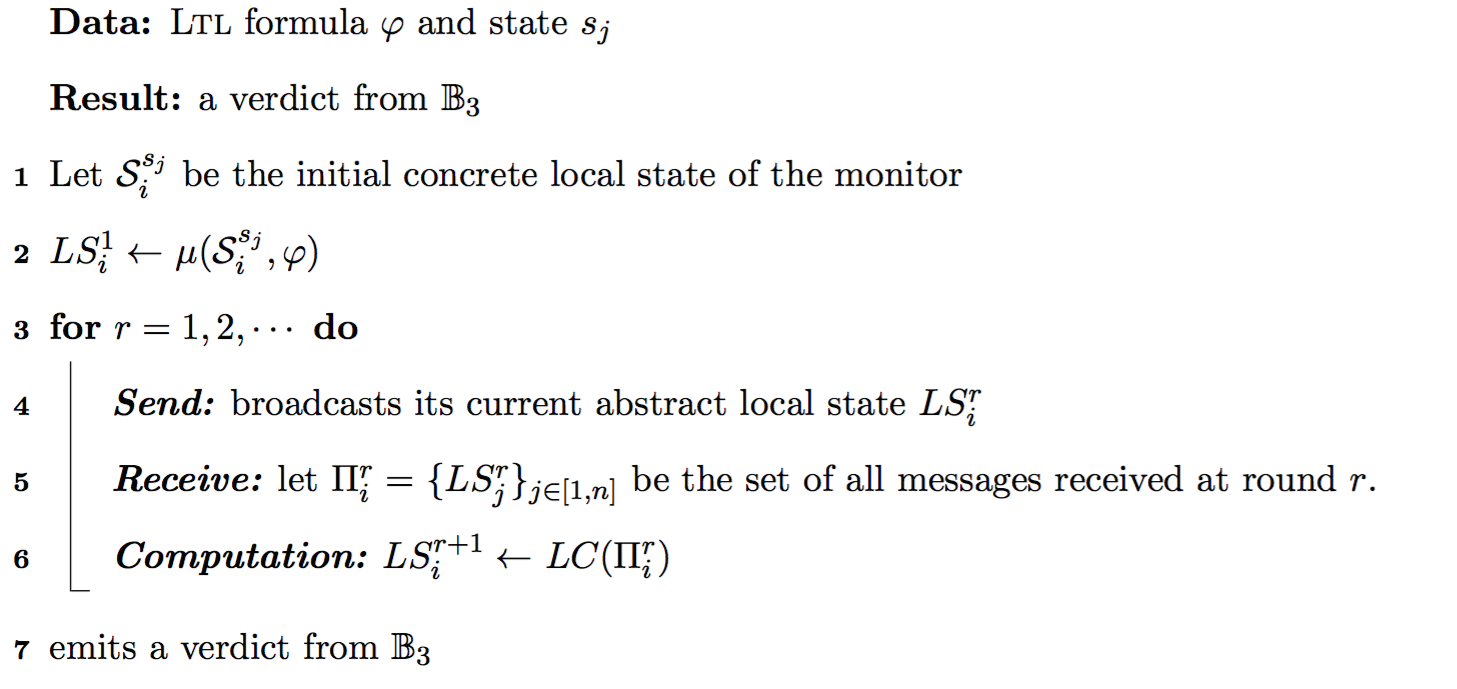
\includegraphics[scale=.3, angle=-360]{figures/synchalgo}
 \end{figure}
 
\begin{block}{Problem Statement}
A non-faulty monitor should compute and emit a verdict that a centralized monitor that has global view of the system would compute. Formally:

$$\forall i \in [1, n] : M_i~ \text{is non-faulty} \; \rightarrow \valuation_i 
= [\alpha \models_3 \varphi]$$ 

\end{block}

\end{block}

 \end{frame}
% ----------------------------------------------------------------------------








\iffalse

Suppose $\fintrace = \state_0\state_1\cdots \state_k$ is a finite trace 
generated by the system under inspection, and $\varphi$ is an \LTL formula with 
respect to which we monitor the system. Each monitor $M_i \in \monitor$, $i \in 
[1, n]$, runs Algorithm \ref{alg:localmonalgo} as follows. For any given new 
state $s_j$, monitor $M_i$ first obtains an initial concrete local state by 
taking a sample from $s_j$ (cf. Line 1). Recall from Definition 
\ref{def:concretestate} that the value of an atomic proposition in a 
concrete local state is either $\tru$, $\fals$, or $\natural$. After obtaining 
the initial concrete local state, monitor $M_i$ computes the initial local 
state based on the initial concrete local state (cf. Line 2). After 
intialization, each monitor $M_i$ executes a sequence of send, receive, and 
computation actions (cf. Lines 4-6) for some a priori known number of rounds.  
In Line 4, monitor $M_i$ sends its current abstract local state to all other 
monitors in $\monitor$. In Line 5, it receives messages from other monitors and 
stores them (along with its own message) in a set $\Pi_i^r$. In line 6, which is 
the computation step, monitor $M_i$ computes and updates its abstract local 
state based on messages in $\Pi_i^r$. Finally, after a certain number of rounds, 
the for-loop ends, and $M_i$ evaluates $\varphi$ and emits a \truthvalue~from 
$\mathbb{B}_3$ based on its final abstract local state (cf. Line 7). Note that 
Algorithm \ref{alg:localmonalgo} is executed whenever a new global state is 
reached in $\fintrace$. 

Our formal problem statement is the termination requirement for Algorithm 
\ref{alg:localmonalgo}. Roughly speaking, we require that when a 
non-faulty monitor runs Algorithm~\ref{alg:localmonalgo} to the end, it should 
compute and emit a verdict that a centralized monitor that has global view of 
the system would compute. This termination condition is formally, the following
$$\forall i \in [1, n] : M_i~ \text{is non-faulty} \; \rightarrow \valuation_i 
= [\alpha \models_3 \varphi]$$ 
where $\valuation_i$ is the \truthvalue~emitted by monitor $M_i$ at the end of 
running Algorithm~\ref{alg:localmonalgo}.


\fi



\section{Related Work}
\begin{frame}{Related Work}
 
\begin{block}{Central Monitor}

\begin{itemize}
\item  H. Chauhan and V. K. Garg and A. Natarajan and N. 
Mittal. \Def{A Distributed Abstraction Algorithm for Online Predicate 
Detection} (SRDS 2013).

\ \\

\item N Mittal and V. K. Garg. \Def{Techniques and applications of computation slicing} (Distributed Computing 2005).

\ \\

\item V. A. Ogale and V. K. Garg. \Def{Detecting Temporal Logic Predicates on Distributed Computations} (DISC 2007).

\end{itemize}
\end{block}

\note{Most existing RV methods employ a central monitor that collects the executions of all components and then checks the system’s global behaviour in terms of a linear- time temporal logic (LTL) formula. The existing work on RV techniques where the monitor consists of a set of components, each having a partial view of the system, is limited to the following}


\end{frame}

% ----------------------------------------------------------------------------
\begin{frame}{Related Work}
 
\begin{block}{Fault-free Setting}

\begin{itemize}


\item A. Bauer and Y. Falcone. \Def{Decentralised {LTL} monitoring} (FMSD 2016).

\ \\

\item C. Colombo and Y. Falcone. \Def{Organising {LTL} monitors over distributed systems with a global clock} (FMSD 2016).

\ \\

\item  M. Mostafa, B. Bonakdarpour. \Def{Decentralized Runtime Verification of 
LTL Specifications in Distributed Systems.} (IPDPS 2015).

%\item Koushik Sen, Abhay Vardhan, Gul Agha, Grigore Rosu:
%\Def{Efficient Decentralized Monitoring of Safety in Distributed Systems.} (ICSE 
%2004)

\end{itemize}
\end{block}

\begin{block}{Fault-tolerant Distributed Monitoring}

B. Bonakdarpour, P. Fraigniaud, S. Rajsbaum, D. A. Rosenblueth, C. Travers. \Def{Decentralized Asynchronous Crash-Resilient Runtime Verification} (CONCUR 2016).

\end{block}


\note{Another short coming of existing RV methods is that they assume a fault-free set- ting, where each individual monitor is resilient to failures. In fact, handling monitors subject to failures, creates significant challenges specially in asynchronous monitoring, as local monitors would not be able to agree on the same perspective of the global system state, due to the impossibility of consensus Fischer et al. (1985). Therefore, it is inevitable that local monitors emit different local verdicts about the current run, and a consistent global verdict with respect to a correctness specification must be constructed from these verdicts. In this area, the work in the literature is limited to Bonakdarpour et al. (2016), where the authors propose a crash-resilient decentral- ized algorithm for monitoring LTL formulas in a wait-free setting.}


\end{frame}



\section{Contributions}
\begin{frame}{Contributions}

\begin{block}{Contributions}
\begin{itemize}

\item An \Def{automata-based} distributed \LTL monitoring algorithm for the decentralized crash-resilient synchronous monitoring.

\ \\

\item Reducing the \Def{message size} overhead from $|\AP|$ per message, to $\log(m_\monstate)$, where $m_\monstate$ is the number of outgoing transitions from the current monitor state in each local monitor's automaton. 

\ \\

\item Introducing an \Def{Extended \LTLtri} monitor for synchronous/asynchronous crash-resilient monitoring.


\end{itemize}
\end{block}
\end{frame}


\section{Synchronous Monitoring}

%-------------------------------------------------------------------------


\iffalse
\begin{frame}{Synchronous Monitoring}


An \LTLtri monitor can evaluate an \LTL formula $\varphi$ in a centralized 
setting where each proposition represents the global state of the system. We 
show in Section \ref{sec:DSM} and Chapter \ref{chap:DAM} that in a framework of several synchronous or asynchronous 
{\em unreliable} monitors, naive local monitoring may lead to inconsistent 
global verdicts for $\varphi$. 

\note{ we propose a framework for synchronous distributed 
fault-tolerant runtime verification (RV). To this end, we make a link between 
RV and consensus in a failure-prone distributed environment by 
proposing an automata-based algorithm.
}

\end{frame}

\fi


\begin{frame}{Synchronous Monitoring}

\begin{block}{Distributed Synchronous Setting}
Finite trace $\alpha = s_0 s_1 \cdots s_k$ ;\\
Set of synchronous monitors $\monitor =\{M_1, M_2, \cdots , M_n\}$ ;\\
Correctness property expressed by an \LTL formula $\varphi$.

\note{1. In the decentralized synchronous setting, we assume the system under scrutiny 
generates a finite trace $\alpha = s_0 s_1 \cdots s_k$ and is inspected by a set 
of synchronous monitors $\monitor =\{M_1, M_2, \cdots , M_n\}$ with respect to 
a correctness property expressed by an \LTL formula $\varphi$. The monitors 
communicate with each other by sending and receiving messages in 
{\em synchronous rounds}, and through point-to-point bidirectional reliable 
communication links. The decentralized crash-resilient synchronous monitoring 
can be reduced to the uniform consensus problem in the crash failure 
model.\\ }

\end{block}

\begin{block}{Algorithm Sketch}
\begin{enumerate} 

\item takes a \Def{sample} from state $s_j$;

\note{\Def{2-reads} the value of a subset of propositions in $s_j$, which may 
result in a {\em partial} observation of $s_j$.\\}

\item \Def{broadcasts} a message containing its current observation, and \Def{receives} messages from other monitors;

\note{\Def{3-at every} synchronous round, {\em broadcasts} a message containing its 
current observation of the underlying system, and then waits for messages from 
other monitors.\\}

\item performs a \Def{local computation} and updates its current observation;

\note{\Def{4-based on the messages received} at each round, executes a local 
computation, updates its current observation by incorporating observations of 
other monitors, and composing the message to be sent at next round.\\}

\item \Def{emits} a truth value from $\mathbb{B}_3$.

\note{\Def{5-finally evaluates} $\varphi$ at the end of communication rounds and 
subsequently emits a truth value from $\mathbb{B}_3$. }

\end{enumerate}

\end{block}

\end{frame}




\begin{frame}{Synchronous Monitoring}

\begin{block}{Uniform Consensus}
Eeach process proposes a value, and the processes have to collectively agree on the same value. 


\begin{itemize}
\item {\bf Validity:} \ A decided value is a proposed value.

\item {\bf Agreement:} \ No two processes decide different values.

\item {\bf Termination:} \ Every correct process decides.
\end{itemize}
\end{block}

\begin{block}{Validity Specification in Synchronous Monitoring}

The decided value must be the same value that a centralized monitor with full 
view of the system would compute.

\end{block}

\begin{block}{Number of Rounds}
The lower bound on the number of rounds required to consistently monitor the system is $f+1$, where $f$ is the total number of crashes the system can tolerate.

\note{It is easy to see that our decentralized synchronous monitoring problem, 
described in Section~\ref{sec:PS}, is similar to the uniform consesus problem that was described in Section \ref{sec:introDSM}. It is also straightforward to verify that the lower bound on the number of rounds required to consistently monitor the system is $f+1$, where $f$ is the total number of crashes the system can tolerate. The proof would be similar to 
the proof of the lower bound on the number of rounds required for the consensus 
algorithm that copes with $f$ process crashes.

}



\end{block}



\note{In the consensus problem, each process proposes a value, and the processes 
have to collectively agree on the same value. Of course, a process can crash 
before deciding a value. Moreover, in order to be meaningful, the value that is 
decided has to be related to the values that are proposed. This is captured by 
the following specification.}





\note{
The validity and agreement properties define the safety property of the 
consensus problem. Validity relates the output to the inputs, while agreement 
captures the difficulty of the problem. Termination is the liveness property of 
the consensus problem. It states that at least the processes that do not crash 
have to decide. In a synchronous setting and in the presence of faults, 
consensus is solvable in $f+1$ rounds, where $f$ is the maximum number of 
processes than can crash.

In the synchronous monitoring problem, the validity specification is that the 
decided value must be the same value that a centralized monitor that has full 
view of the system would compute.
}







\end{frame}




\begin{frame}{Synchronous Monitoring}

\begin{block}{Local Monitor Algorithm}

\begin{figure}
 \centering
 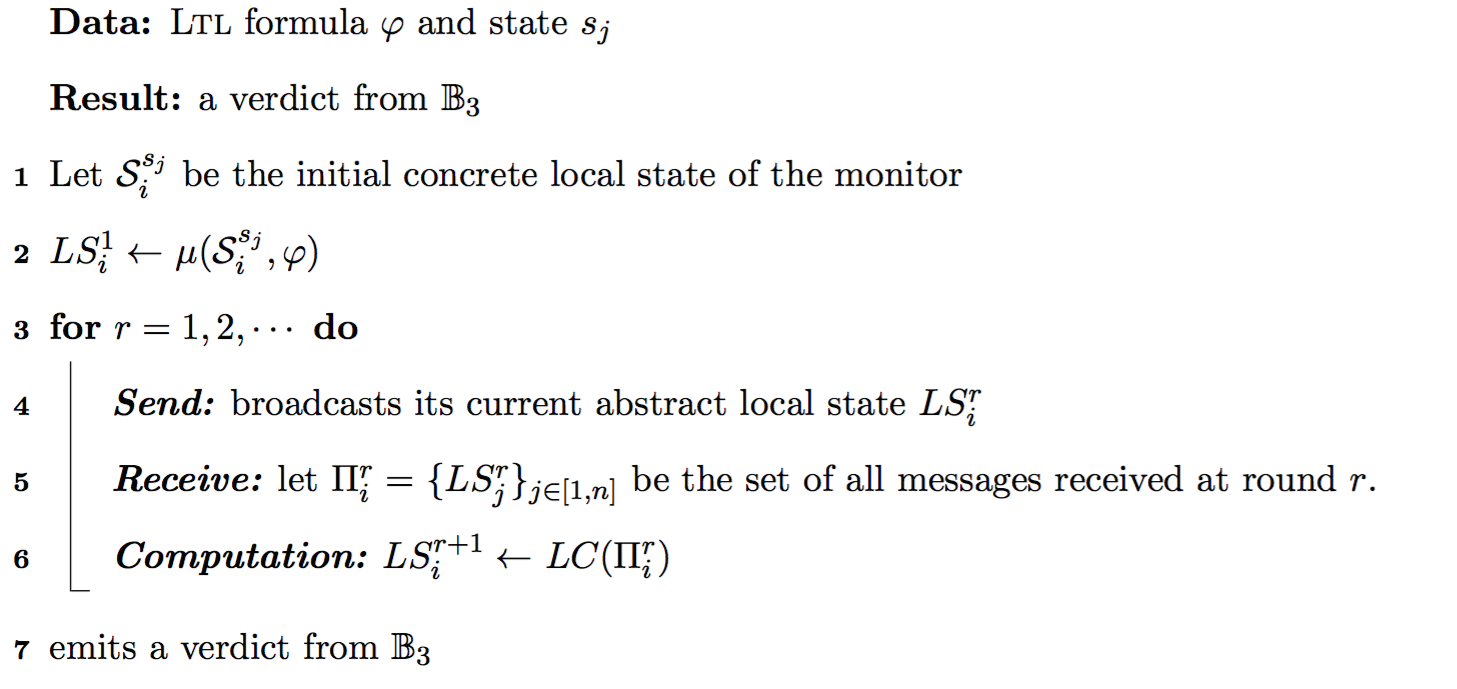
\includegraphics[scale=.3, angle=-360]{figures/synchalgo}
 \end{figure}

\end{block}

\end{frame}



\begin{frame}{Challenges in Synchronous Monitoring}


\begin{example}
Let $\varphi = \F (a \, \wedge \, b)$, $\AP=\{a, b\}$, and $\monitor =\{M_1, 
M_2, M_3, M_4\}$. Suppose $s=\{a,b\}$ is the current global state of the 
system, and the initial samples of the monitors are as follows:\\


\begin{center}

\begin{tabular}{| c |c |c|}

\multicolumn{3}{c}{sample} \\
\hline
&$a$&$b$\\
\hline
$M_1$ & $\tru$  & $\natural$\\
$M_2$ & $\natural$ & $\tru$\\
$M_3$ & $\natural$ & $\tru$ \\
$M_4$ & $\natural$ & $\tru$ \\
%$M_5$ & $\natural$ & $true$ \\
\hline
\end{tabular}
\quad
\begin{tabular}{| c |c |c|}
\multicolumn{3}{c}{round 1} \\
\hline
&$a$&$b$\\
\hline
$M_1$ & crashed & crashed\\
$M_2$ & $\tru$ & $\tru$\\
$M_3$ & $\natural$ & $\tru$ \\
$M_4$ & $\natural$ & $\tru$ \\
%$M_5$ & $\natural$ & $true$ \\
\hline
\end{tabular}


\end{center}


\begin{center}
\begin{tabular}{|c |c |c|}
\multicolumn{3}{c}{round 2} \\
\hline
&$a$&$b$\\
\hline
$M_1$ & crashed & crashed\\
$M_2$ & crashed & crashed\\
$M_3$ & $\tru$ & $\tru$ \\
$M_4$ & $\natural$ & $\tru$ \\
%$M_5$ & $\natural$ & $true$ \\
\hline
\end{tabular}
\quad
\begin{tabular}{| c |c |c|}
\multicolumn{3}{c}{round 3} \\
\hline
&$a$&$b$\\
\hline
$M_1$ & crashed & crashed\\
$M_2$ & crashed & crashed\\
$M_3$ & $\tru$ & $\tru$  \\
$M_4$ & $\tru$ & $\tru$  \\
%$M_5$ & $true$ & $true$  \\
\hline
\end{tabular}   

\end{center}

\end{example}
 
\end{frame}


\begin{frame}{Synchronous Monitoring}
\begin{block}{Challenge}

If each monitor broadcasts its sample ~$\Rightarrow$ ~ the message size is \Def{$|\AP|$}

\end{block}


\begin{block}{Reducing the Message Size Overhead}
We introduce an algorithm which decreases the message size from $|\AP|$ to  \Def{$\log(m_\monstate)$} where $m_\monstate$ is the number of outgoing transitions from monitor state $\monstate$.

\end{block}





\note{One can see in the above example, in case each monitor broadcasts its concrete 
local state, namely, if the abstract local state is the same as the concrete 
local state, then each message sent by a monitor is a register that consists of 
$|\AP|$ elements, one for each atomic proposition in $\AP$. Our goal is to 
decrease the message size overhead, hence we introduce an algorithm that 
decreases the message size from $|\AP|$ bits to something 
significantly lower. In Section \ref{sec:SAM}, we introduce an algorithm which 
decreases the message size overhead in synchronous distributed monitoring. The 
algorithm solves the synchronous distributed monitoring problem in $f +1$ 
rounds of communication with message size of $\log(m_\monstate)$, where $m_\monstate$ is the number of outgoing transitions from monitor state $\monstate$ in an \Exltl~that will be introduced in Section \ref{sec:SAMExltl}.
}



\end{frame}


\begin{frame}{Automata-based Synchronous Monitoring}

\begin{block}{The General Idea}

\begin{itemize}

\item Each local monitor $M_i$ evaluates the input formula and computes a \Def{possible} set of verdicts;

$$\verdict_i = \{\delta(\monstate, s') \mid s' \in 
\pevent(\sample_i^s)\}$$ \\


\note{Each \Def{possible verdict} is a monitor state that can be reached by a possible global state from viewpoint of monitor $M_i$.}


\item At each round, each monitor $M_i$ broadcasts its verdict set $V_i$, and computes a new verdict set by applying the \Def{intersection} function on the verdict sets received from other monitors;

$$\verdict_i^{r+1} = LC(\Pi_i^r) = \bigcap_{j \in [1, n]} \{ \verdict_j^r\} = 
\bigcap_{j \in [1, n]} \{\verdict_j^r\}$$


\item After $f+1$ rounds of communication, each monitor emits the verdict that a centralized monitor that has the global view of the system would compute.


\end{itemize}

\end{block}

\end{frame}



\begin{frame}{Automata-based Synchronous Monitoring}

\begin{block}{Local Monitor Algorithm}

\begin{figure}
 \centering
 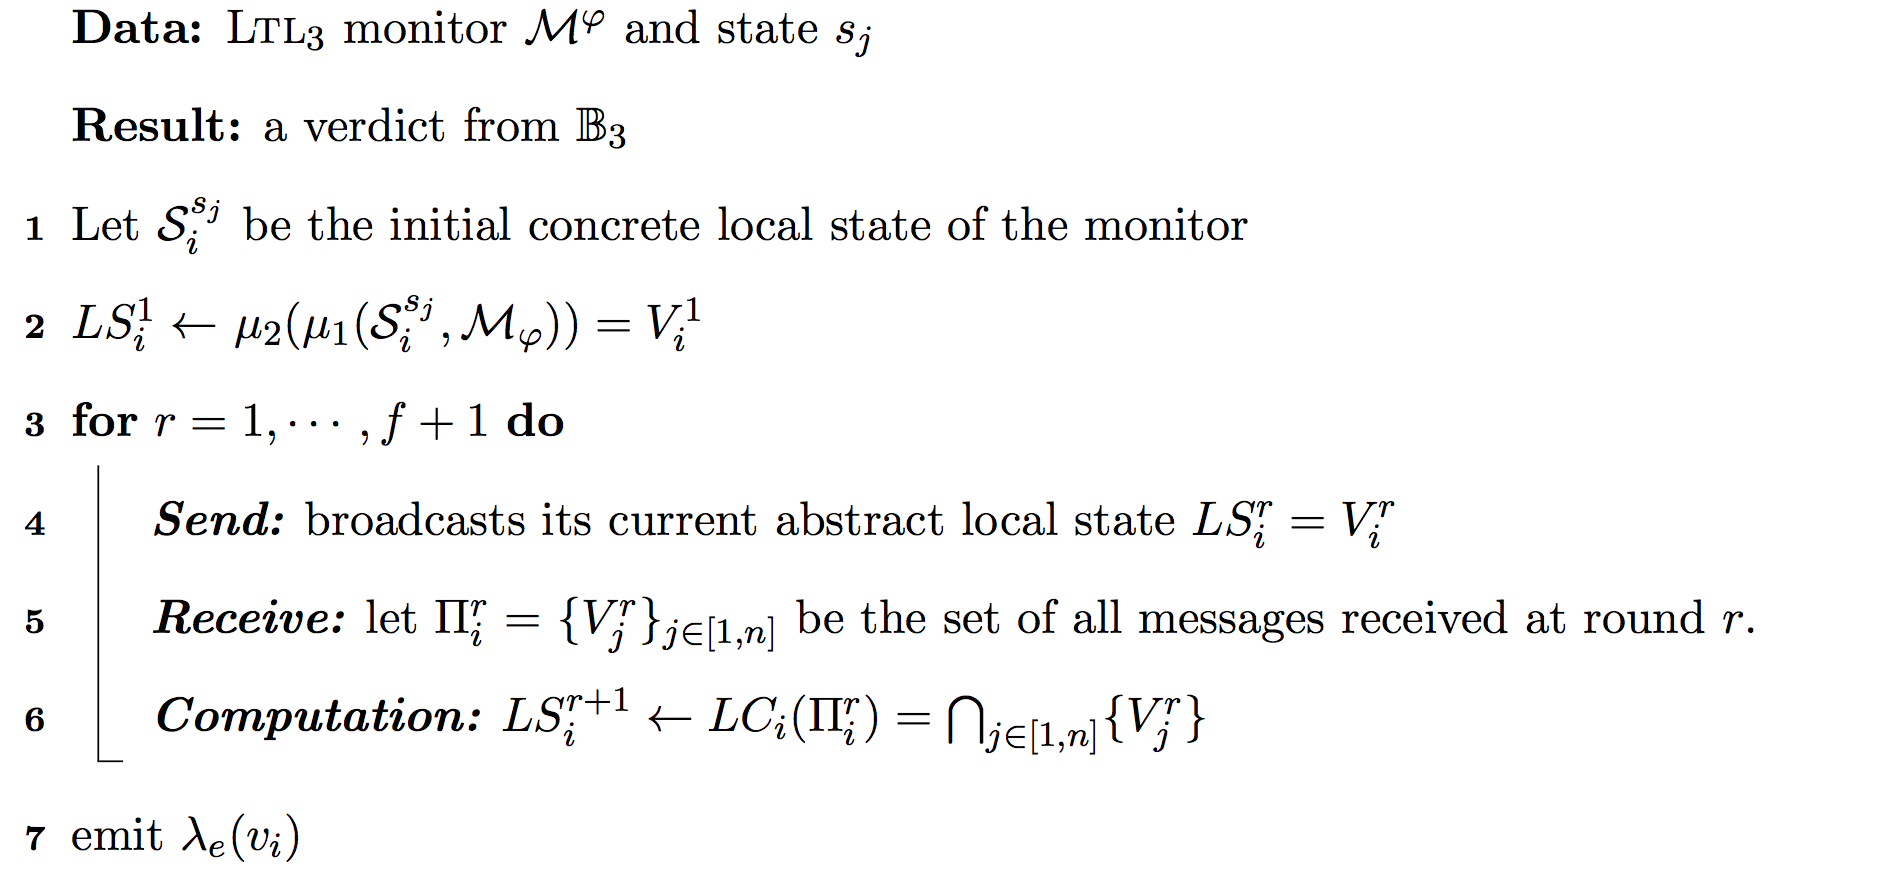
\includegraphics[scale=.3, angle=-360]{figures/localmonalgo2}
 \end{figure}

\end{block}

\end{frame}





\begin{frame}{Automata-based Synchronous Monitoring}

\begin{example}

Let $\varphi = \F (a \wedge b)$.

\begin{figure}[H]
\centering
\begin{tikzpicture}[->,>=stealth',shorten >=1pt,auto,node distance=4.8cm,
                    semithick, initial text={}, initial where=right]
  \tikzstyle{every state}=[scale=0.65, every node/.style={scale=0.65}]

  \node[initial,state] (A)                {$\monstate_0$};
  \node[state, accepting]         (B) [left of  = A] {$\monstate_\top$};

  \path (A) edge              node {$ \{a,b\}$} (B)
 
            edge [loop above] node {$\{a\}, \{b\}, \emptyset$} (A) ;
        
\end{tikzpicture}    
\caption{\LTLtri monitor of $\varphi = \F(a \wedge b)$.}
\end{figure}

And suppose the initial samples of the monitors are as follows:

\begin{center}

\begin{tabular}{| c |c |c |c|}
\multicolumn{3}{c}{sample} \\
\hline
&$a$&$b$&$\verdict_i^1$\\
\hline
$M_1$ & $\tru$  & $\natural$ & $\{\monstate_0, \monstate_\top\}$\\
$M_2$ & $\natural$ & $\tru$ &  $\{\monstate_0, \monstate_\top\}$\\
$M_3$ & $\natural$ & $\natural$ &  $\{\monstate_0, \monstate_\top\}$ \\
$M_4$ & $\natural$ & $\natural$ &  $\{\monstate_0, \monstate_\top\}$\\
%$M_5$ & $\natural$ & $true$ \\
\hline
\end{tabular} 

\end{center}

\end{example}

\end{frame}




\begin{frame}{Automata-based Synchronous Monitoring}

\begin{example}

\begin{center}
\begin{tabular}{| c |c|}
\multicolumn{2}{c}{round 1} \\
\hline
&$\verdict_i^2$\\
\hline
$M_1$ & crashed\\
$M_2$ & $\{\monstate_0, \monstate_\top\}$\\
$M_3$ & $\{\monstate_0, \monstate_\top\}$ \\
$M_4$ & $\{\monstate_0, \monstate_\top\}$ \\
%$M_5$ & $\natural$ & $true$ \\
\hline
\end{tabular}
\quad
\begin{tabular}{| c |c|}
\multicolumn{2}{c}{round 2} \\
\hline
&$\verdict_i^3$\\
\hline
$M_1$ & crashed\\
$M_2$ & crashed\\
$M_3$ & $\{\monstate_0, \monstate_\top\}$ \\
$M_4$ & $\{\monstate_0, \monstate_\top\}$ \\
%$M_5$ & $\natural$ & $true$ \\
\hline
\end{tabular}
\quad
\begin{tabular}{| c |c|}
\multicolumn{2}{c}{round 3} \\
\hline
&$\verdict_i^4$\\
\hline
$M_1$ & crashed\\
$M_2$ & crashed\\
$M_3$ & $\{\monstate_0, \monstate_\top\}$ \\
$M_4$ & $\{\monstate_0, \monstate_\top\}$ \\
%$M_5$ & $\natural$ & $true$ \\
\hline
\end{tabular} 
\end{center}

As we see $|\verdict_3|=|\verdict_4| > 1$. Therefore, they cannot emit the correct verdict $\top$  as  we have $[\{a, b\} \models_3 \F(a \wedge b)] = \top$.
\end{example}

\begin{block}{Insufficiency of \LTLtri Monitor}
The \LTLtri monitor of $\varphi = \F (a \wedge b)$ is not sufficient to distinguish 
the correct verdict when local monitors have partial view of the system.


\note{As we observe, at the end of round $3$ (namely, $f+1$), the local monitors still 
cannot decide a single verdict since $|\abstate_i^4| > 1$. This is because the 
\LTLtri monitor of $\varphi = \F (a \wedge b)$ is not sufficient to distinguish 
the correct verdict when local monitors have partial view of the system. In 
particular, monitors $M_3$ and $M_4$ both have $\{\monstate_0, 
\monstate_\top\}$ as their verdicts, while $[\{a, b\} \models_3 \F(a 
\wedge b)] = \top$. That is, the monitors cannot map their collective verdicts 
to the verdict of a monitor that has the global view of the system. 


In order to resolve this insufficiency, we introduce an algorithm that 
constructs an `\Exltl'. The algorithm receives as input an \LTLtri monitor and 
solely based on the structure of the input monitor, it determines whether to add 
new monitor states to the original \LTLtri monitor. The \Exltl~then is used in 
each local monitor $M_i$'s algorithm (Algorithm \ref{alg:localmonalgo2}) to 
consistently solve the decentralized synchronous monitoring problem. As 
described earlier, the intuition behind this algorithm is to monitor the system 
under inspection by taking the intersection of the sets of verdicts emitted by a 
set of distributed monitors. }

\end{block}


\end{frame}




\begin{frame}{Automata-based Synchronous Monitoring}
\begin{block}{Extended \LTLtri Monitor}


\textbf{Input:} \LTLtri monitor  $\monitor^\varphi = \{ \alphabet, Q, \monstate_0, \delta , \lambda\}$ 

\textbf{output:}  Extended \LTLtri monitor $\monitor^\varphi_e = \{ \alphabet, Q_e, 
\monstate_0, \delta_e , \lambda_e\}$

Where, 

\ \\

$Q \subseteq Q_e$, $q_0$ \\
$q_0$ is the initial state\\
$\delta_e: Q_e \times \alphabet \rightarrow 2^{Q_e}$ is a transition function\\
$\lambda_e : Q_e \rightarrow \mathbb{B}_3 $ is a mapping function, such that: 

\ \\

\begin{enumerate}

\item for every non-empty finite trace $\alpha \in \alphabet^*$, we have $\lambda_e 
(\delta_e(q_0, \alpha)) = \lambda (\delta(q_0, \alpha))$.

\item at every 
$\monstate \in Q_e$ we have $|\intersection| = 1$. 

%Where $|\intersection|$ is the intersection of all verdict sets emitted  by local monitors.

\end{enumerate}

\end{block}
\end{frame}

\note{Let $\monitor^\varphi = \{ \alphabet, Q, \monstate_0, \delta , \lambda\}$ be the 
\LTLtri monitor of an \LTL formula $\varphi$. An {\em \Exltl}~of $\varphi$ is a 
deterministic finite state machine $\monitor^\varphi_e = \{ \alphabet, Q_e, 
\monstate_0, \delta_e , \lambda_e\}$, where $Q_e$ is a set of states s.t. $Q 
\subseteq Q_e$, $q_0$ is the initial state, $\delta_e: Q_e \times \alphabet 
\rightarrow 2^{Q_e}$ is a transition function, and $\lambda_e : Q_e 
\rightarrow \mathbb{B}_3 $ is a mapping function, such that (1) for every 
non-empty finite trace $\alpha \in \alphabet^*$, we have $\lambda_e 
(\delta_e(q_0, \alpha)) = \lambda (\delta(q_0, \alpha))$, and (2) at every 
$\monstate \in Q_e$ we have $|\intersection| = 1$.}







\begin{frame}{Extended \LTLtri Monitor Construction}


\begin{block}{Transition}

A transition $t_j^i$ from monitor state $\monstate_i$ to monitor 
state $\monstate_j$ is defined as follows:
$$ t_j^i = \{ \state \in \alphabet ~ | ~ \delta (\monstate_i, \state) = 
\monstate_j\}$$

\end{block}



\begin{block}{Indistinguishable Transitions}

We say a transition $t_1$ is \Def{indistinguishable} from another transition 
$t_2$, and denote it by $\indisting(t_1, t_2)$, if the following holds: 
 
$$\exists \state \in t_2 . ~ \dep(\state, t_1)$$

\end{block}



\begin{block}{Covered State}


We say state $\state$ is \Def{covered} by transition $t$, and we denote it 
by $\dep(\state, t)$, if we have:

$$ \forall \ap \in \AP.~ \exists \state' \in t. ~(\ap \in \state 
\Leftrightarrow \ap \in \state') $$

\end{block}


\end{frame}





\begin{frame}{Extended \LTLtri Monitor Construction}

\vspace{-1mm}
\begin{figure}
 \centering
 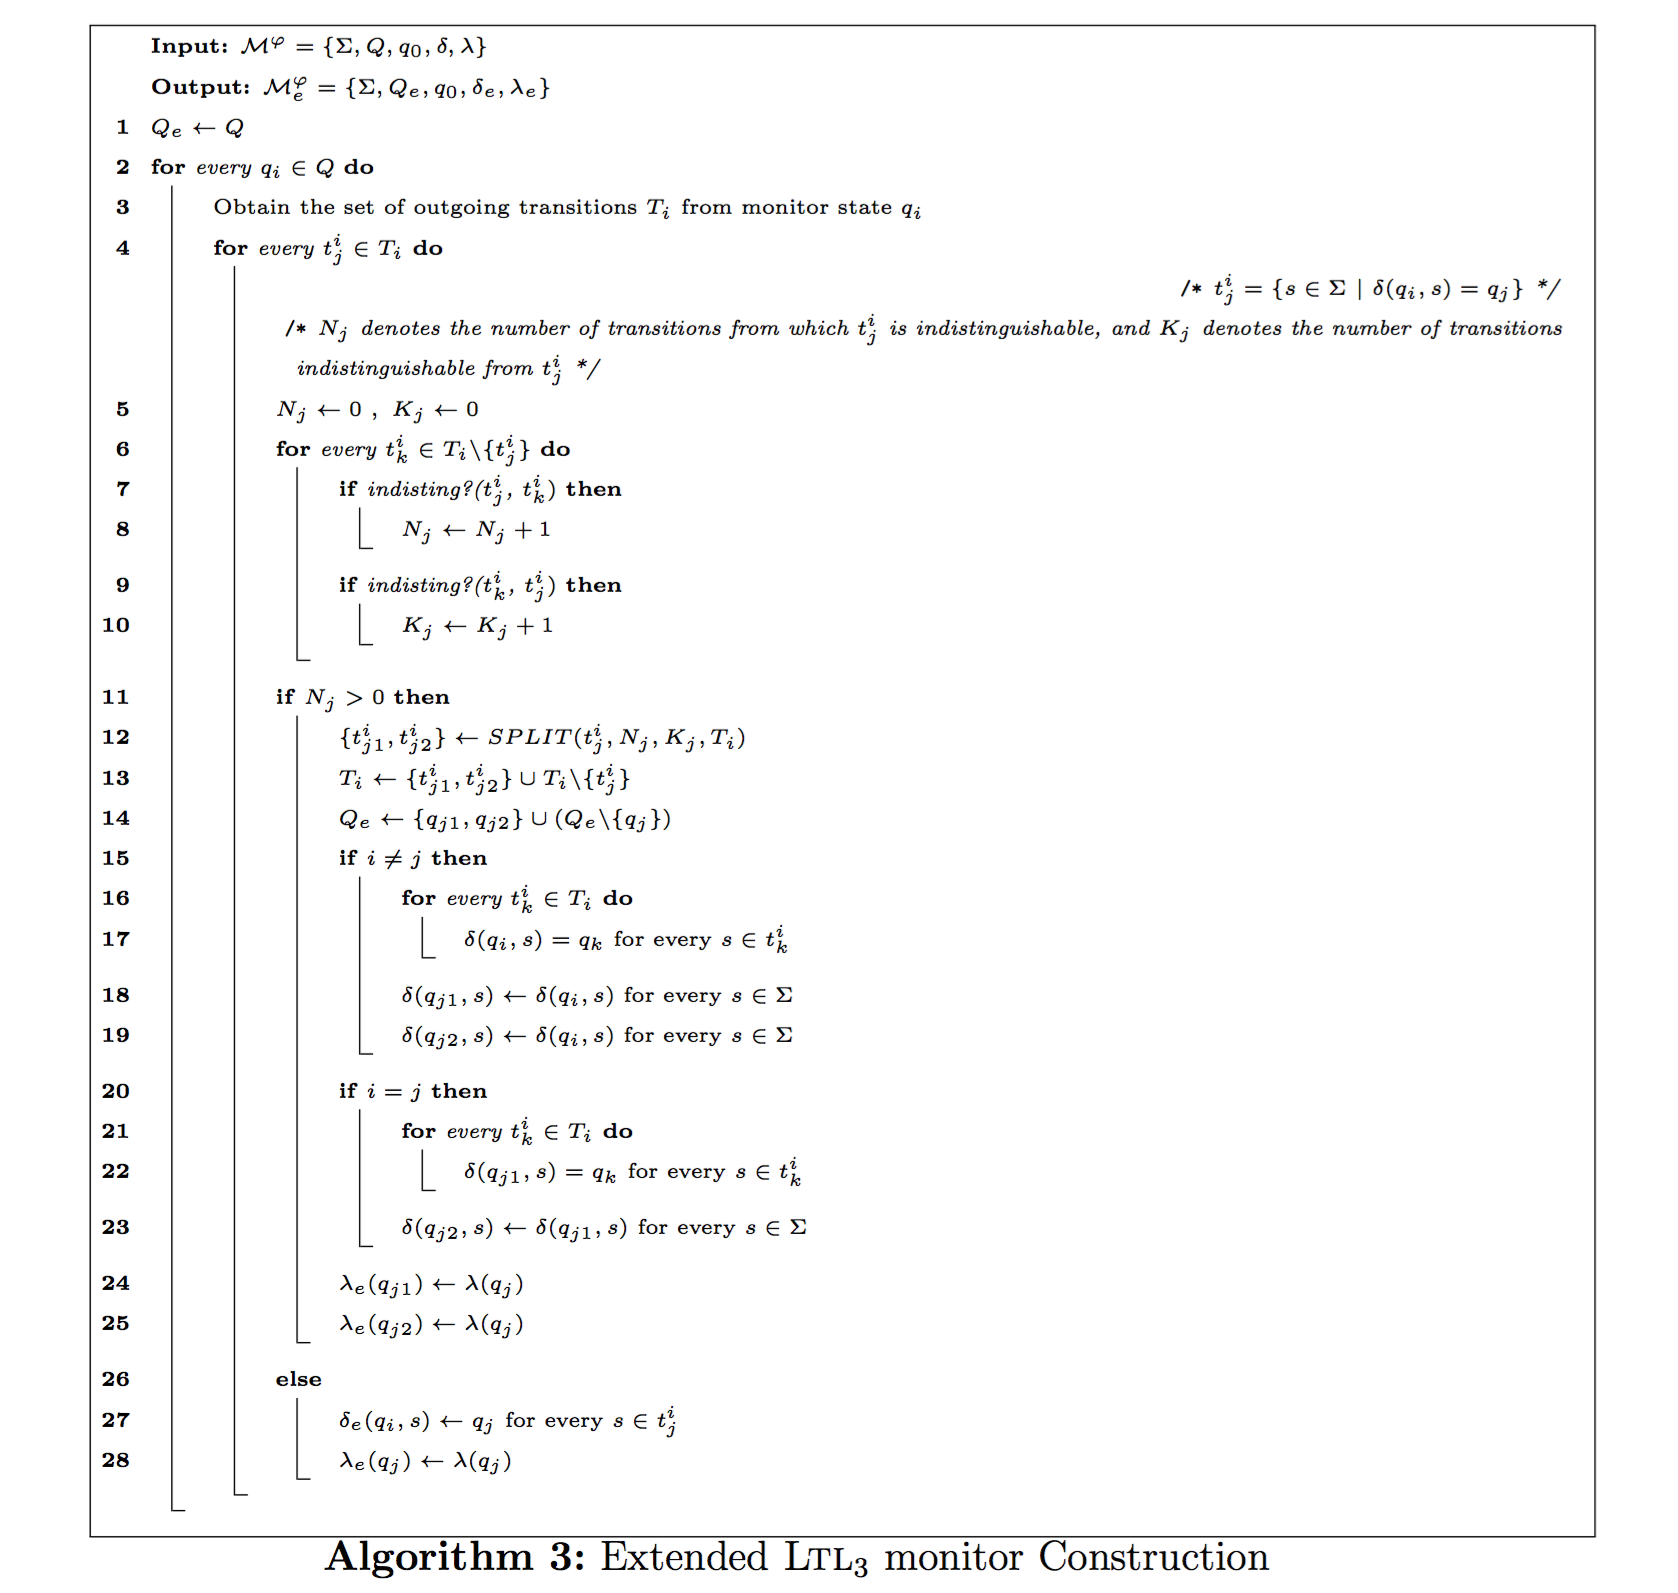
\includegraphics[scale=.25, angle=-360]{figures/ExltlMon}
 \end{figure}

 \end{frame}
 





\begin{frame}{Automata-based Synchronous Monitoring}


\begin{example}


Consider the \LTLtri monitor for $\varphi = \F (a \wedge b)$. 

%We have $\monitor^\varphi = \{ \{a, b\}, \{\monstate_0, \monstate_\top\}, \monstate_0, \delta, \lambda   \}$, where \\

\ \\

%$\delta(\monstate_0, \{a\}) = \delta(\monstate_0, \{b\}) = \delta(\monstate_0, \emptyset) = \monstate_0$  \\
%$\delta(\monstate_0, \{a, b\}) = \monstate_\top$. 




\iffalse
The set of outgoing 
transitions from monitor state $\monstate_0$ is $T_0 = \{t_0^0, t_\top^0\}$, 
where  $t_0^0 = \{\{a\}, \{b\}, \emptyset\}$ and $t_\top^0 = \{\{a,b\}\}$ are 
the outgoing transitions from monitor state $\monstate_0$ to monitor states 
$\monstate_0$ and $\monstate_\top$, respectively. We can verify that transition 
$t_0^0$ is \indist~from $t_\top^0$ since there is a state $\{a, b\} \in 
t_\top^0$ that is \covered~by transition $t_0^0$, i.e., $\dep (\{a, b\}, t_0^0) 
= \tru$. But $t_\top^0$ is not \indist~from $t_0^0$. Therefore, we have $N_0 = 
1$, $K_0 = 0$, $N_\top = 0$, and $K_\top = 0$. Since $N_0 > 0$, we \splt~$t_0^0$ 
into two transitions $t_{01}^0$ and $t_{02}^0$. Different \partitionn s of 
$t_0^0$ are as follows: 
\fi




\begin{figure}[H]
\centering

\begin{tikzpicture}[->,>=stealth',shorten >=1pt,auto,node distance=4.8cm,
                    semithick, initial text={}, initial where=right]
  \tikzstyle{every state}=[scale=0.65, every node/.style={scale=0.65}]

  \node[initial,state] (A)                {$\monstate_0$};
  \node[state, accepting]         (B) [left of  = A] {$\monstate_\top$};
 
  \path (A) edge              node {$ \{a,b\}$} (B)
     
            edge [loop above] node {$\{a\}, \{b\}, \emptyset$} (A) ;
  \path  (B) edge [loop above] node {$\tru$} (B);          
\end{tikzpicture}    
%\caption{$\monitor^\varphi$}
\end{figure}

The set of outgoing transitions from monitor state $q_0$ is $T_0 = \{t_0^0, t_\top^0\}$ where: 

\ \\ 

$t_0^0 = \{\{a\}, \{b\}, \emptyset\}$  \\
$t_\top^0 = \{\{a,b\}\}$

\ \\

We can verify that $t_0^0$ is indistinguishable from $t_\top^0$. Therefore we split transition $t_0^0$ into two transitions $t_{01}^0 = \{\{a\}\}$ and $t_{02}^0 = \{\{b\}, \emptyset\}$.


\end{example}

\end{frame}








\begin{frame}

\begin{example}


\begin{figure}[H]
\centering

\begin{tikzpicture}[->,>=stealth',shorten >=1pt,auto,node distance=4.8cm,
                    semithick, initial text={}, initial where=right]
  \tikzstyle{every state}=[scale=0.65, every node/.style={scale=0.65}]

  \node[state, visible on=<1->] (A)                {$\monstate_{01}$};
  \node[state, accepting, visible on=<1->]         (B) [left of  = A] {$\monstate_\top$};
  \node[state, visible on=<1->]         (D) [below of = B] {$\monstate_{02}$};

  \path (A) edge   [visible on=<1->]           node {$ \{a,b\}$} (B)
                 edge [loop above, visible on=<2->] node {$\{b\}, \emptyset$} (A)
                 edge      [bend left=20, visible on=<2->]     node   {$\{a\}$} (D)
        (B) edge [loop above, visible on=<1->] node {$\tru$} (B)
        (D) edge [visible on=<3->]                node {$\{a,b\}$} (B)
        (D) edge       [bend left=15, visible on=<3->]             node {$\{b\}, \emptyset$} (A)
        (D) edge [loop below, visible on=<3->] node {$\{a\}$} (D);

\end{tikzpicture}    
\end{figure}


Note that we have

\begin{center}
$\lambda(\monstate_{01}) = \lambda(\monstate_0) = ?$\\
$\lambda(\monstate_{02}) = \lambda(\monstate_0) = ?$
\end{center}


\end{example}

\end{frame}



\begin{frame}{Automata-based Synchronous Monitoring}

\begin{example}


Suppose $s=\{a,b\}$ is the current global state of the system and Let $\varphi = \F (a \wedge b)$. The initial state of the monitors is as follows:\\


\begin{center}

\begin{tabular}{| c |c |c |c|}
\multicolumn{3}{c}{sample} \\
\hline
&$a$&$b$&$\abstate_i^1$\\
\hline
$M_1$ & $\tru$  & $\natural$ & $\{\monstate_{02}, \monstate_\top\}$\\
$M_2$ & $\natural$ & $\tru$ &  $\{\monstate_{01}, \monstate_\top\}$\\
$M_3$ & $\natural$ & $\natural$ &  $\{\monstate_{01},\monstate_{02}, 
\monstate_\top\}$ \\
$M_4$ & $\natural$ & $\natural$ &  $\{\monstate_{01}, \monstate_{02}, 
\monstate_\top\}$\\
%$M_5$ & $\natural$ & $true$ \\
\hline
\end{tabular} 
\quad
\begin{tabular}{| c |c|}
\multicolumn{2}{c}{round 1} \\
\hline
&$\abstate_i^2$\\
\hline
$M_1$ & crashed\\
$M_2$ & $\{\monstate_\top\}$\\
$M_3$ & $\{\monstate_{01}, \monstate_\top\}$ \\
$M_4$ & $\{\monstate_{01}, \monstate_\top\}$ \\
%$M_5$ & $\natural$ & $true$ \\
\hline
\end{tabular}
\end{center}

\begin{center}

\begin{tabular}{| c |c|}
\multicolumn{2}{c}{round 2} \\
\hline
&$\abstate_i^3$\\
\hline
$M_1$ & crashed\\
$M_2$ & crashed\\
$M_3$ & $\{\monstate_\top\}$ \\
$M_4$ & $\{\monstate_{01}, \monstate_\top\}$ \\
%$M_5$ & $\natural$ & $true$ \\
\hline
\end{tabular} 
\quad
\begin{tabular}{| c |c|}
\multicolumn{2}{c}{round 3} \\
\hline
&$\abstate_i^4$\\
\hline
$M_1$ & crashed\\
$M_2$ & crashed\\
$M_3$ & $\{\monstate_\top\}$ \\
$M_4$ & $\{\monstate_\top\}$ \\
%$M_5$ & $\natural$ & $true$ \\
\hline
\end{tabular} 
\end{center}




\end{example}

\end{frame}






\section{Asynchronous Monitoring}

%-------------------------------------------------------------------------
\begin{frame}{Asynchronous Monitoring}



\note{each local monitor obtains a partial view (i.e., a concrete local state) of the system's global state. It communicates with other monitors through a shared memory and updates its knowledge, and then solely based on its partial view, emits a final verdict. We show how, given any \LTL formula and an \Exltl, a set of verdicts collectively provided by the local monitors can be used to compute the verdict computed by a centralized monitor that has full view of the system under scrutiny.}


\begin{block}{Asynchronous Monitoring}

The system under inspection produces a finite trace $\alpha = \state_0 \state_1 \cdots \state_k$, and is inspected with respect to an \LTL formula $\varphi$ by a set $\monitor = \{ M_1, M_2, \cdots , M_n \}$ of asynchronous distributed monitors.

\end{block}


\begin{block}{Local Monitor Algorithm}

\begin{figure}
 \centering
 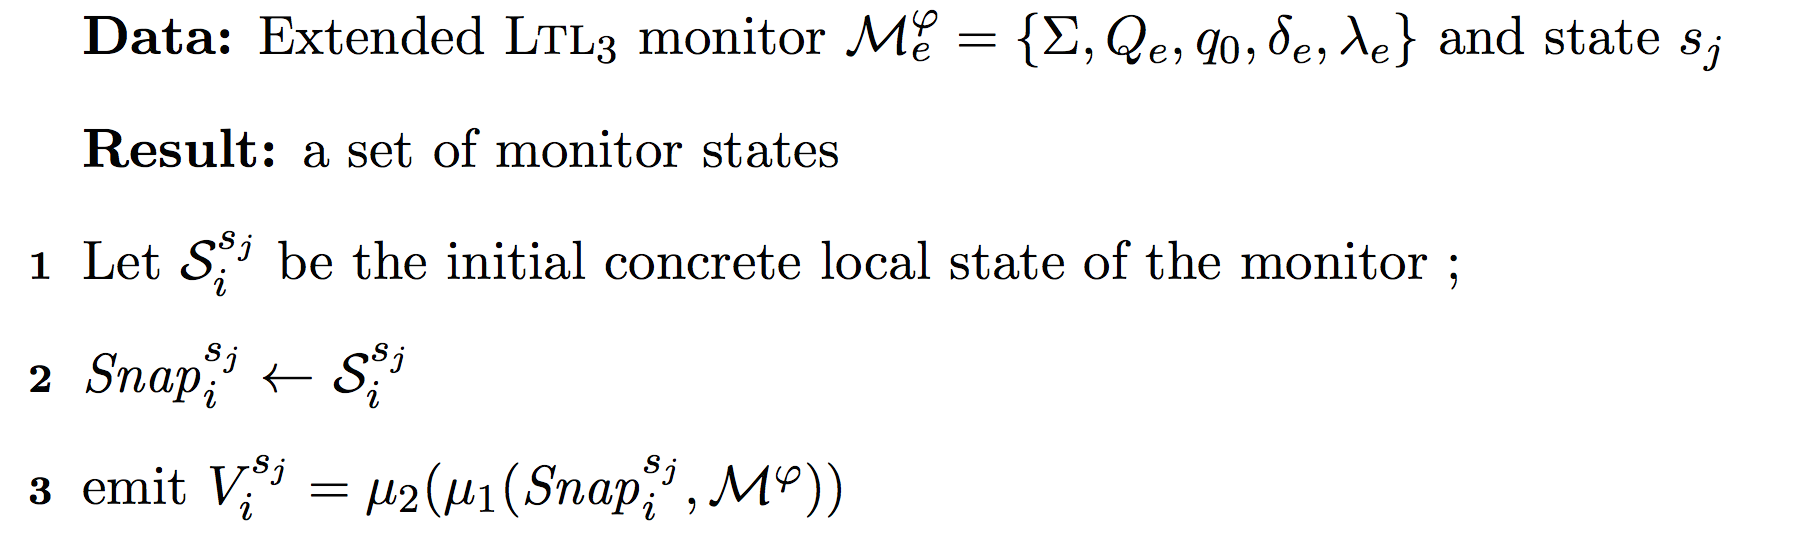
\includegraphics[scale=.25, angle=-360]{figures/asynchalgo}
 \end{figure}


\end{block}

\end{frame}



\begin{frame}{Asynchronous Monitoring}


\begin{example}

 Let $\varphi = \F (a \wedge b)$ whose \Exltl~is given below. Suppose monitors are at monitor state $\monstate_0$, and let $\state= \{a, b\} $ be the global state of the system. \\

\ \\

\begin{figure}[H]
\centering
\begin{tikzpicture}[->,>=stealth',shorten >=1pt,auto,node distance=4.8cm,
                    semithick, initial text={}, initial where=right]
  \tikzstyle{every state}=[scale=0.55, every node/.style={scale=0.65}]

  \node[initial,state] (A)                {$\monstate_0$};
  \node[state, accepting]         (B) [left of  = A] {$\monstate_\top$};
  \node[state]         (D) [below of = B] {$\monstate_1$};

  \path (A) edge              node {$ \{a,b\}$} (B)
                 edge [loop above] node {$\{b\}, \emptyset$} (A)
                 edge      [bend left=20]     node   {$\{a\}$} (D)
        (B) edge [loop above] node {$\tru$} (B)
        (D) edge                 node {$\{a,b\}$} (B)
        (D) edge       [bend left=15]             node {$\{b\}, \emptyset$} (A)
        (D) edge [loop below] node {$\{a\}$} (D);

\end{tikzpicture}    

\end{figure}

\end{example}

\end{frame}



\begin{frame}

\begin{example}
The following tables represent each monitor $M_i$'s initial \localreg~$\snap_i^\state$ and its verdict set $\verdict_i$ calculated based on only $\snap_i^\state$.

\ \\


\begin{center}

 \begin{tabular}{|c|c|c|c|}
   \multicolumn{1}{r}{} &  \multicolumn{2}{c}{ {$\snap_1^\state$}}\\
\hline
  & $M_1$ & $M_2$ & $M_3$\\
 \hline
   $a$ & $\tru$ & $\udef$ & $\udef$\\
   $b$ & $\udef$ & $\udef$ & $\udef$\\
\hline
  $\verdict_1$  &  \multicolumn{3}{c|}{\cellcolor{gray!25}$\{\monstate_1, \monstate_\top\}$}\\
\hline
  \end{tabular}  
\quad
 \begin{tabular}{|c|c|c|c|}
   \multicolumn{1}{r}{} &  \multicolumn{2}{c}{ {$\snap_2^\state$}}\\
\hline
  & $M_1$ & $M_2$ & $M_3$\\
 \hline
   $a$ & $\udef$ & $\udef$ & $\udef$\\
   $b$ & $\udef$ & $\tru$ & $\udef$\\
\hline
  $\verdict_2$  &  \multicolumn{3}{c|}{\cellcolor{gray!25}$\{\monstate_0, \monstate_\top\}$}\\
\hline
  \end{tabular} 
%\quad

\end{center}


\begin{center}
 \begin{tabular}{|c|c|c|c|}
   \multicolumn{1}{r}{} &  \multicolumn{2}{c}{ {$\snap_3^\state$}}\\
\hline
  & $M_1$ & $M_2$ & $M_3$\\
 \hline
   $a$ & $\udef$ & $\udef$ & $\udef$\\
   $b$ & $\udef$ & $\udef$ & $\udef$\\
\hline
  $\verdict_3$  &  \multicolumn{3}{c|}{\cellcolor{gray!25}$\{\monstate_0, \monstate_1, \monstate_\top\}$}\\
\hline
  \end{tabular}   
\end{center}


$\verdict_1 \cap \verdict_2 \cap \verdict_3 = q_\top$.

\end{example}

\end{frame}










\section{Conclusion}
\begin{frame}{Conclusion}

\begin{block}{Conclusion}
\begin{itemize}

\item We proposed a synchronous monitoring algorithm that copes with $f$ crash failures in a distributed setting. The algorithm solves the synchronous monitoring problem in \Def{$f +1$} rounds of communication and reduces the message size overhead from $|\AP|$ to \Def{$\log(m_\monstate)$}.

\ \\

\item We proposed an algorithm for distributed crash-resilient asynchronous RV that \Def{consistently} monitors the system under inspection with \Def{no communication} between monitors. 

\end{itemize}
\end{block}
\end{frame}



\section{Future Work}
\begin{frame}{Future Work}

\begin{block}{Futur Work}
\begin{itemize}

\item To address more severe faults, e.g., Byzantine failures. 

\ \\

\item To have monitors observe, communicate, and emit verdicts between any two global states.

\ \\ 

\item To extend our results to the case where the input to the monitors is a sequence of global states and each monitor produces a sequence of verdict sets, one per each global state


\end{itemize}
\end{block}
\end{frame}




%\input{content/rv-ltl}
%\input{content/dm}
%\input{content/ltlk}
%\input{content/concl}

\end{document}